\cleardoublepage
\chapter{\secState{R}Approach}\label{ch:approach}

\noindent There levels of \emph{Avoidance} are summarized in (fig. \ref{s:approachOverview}).

\begin{figure}[H]
    \centering
    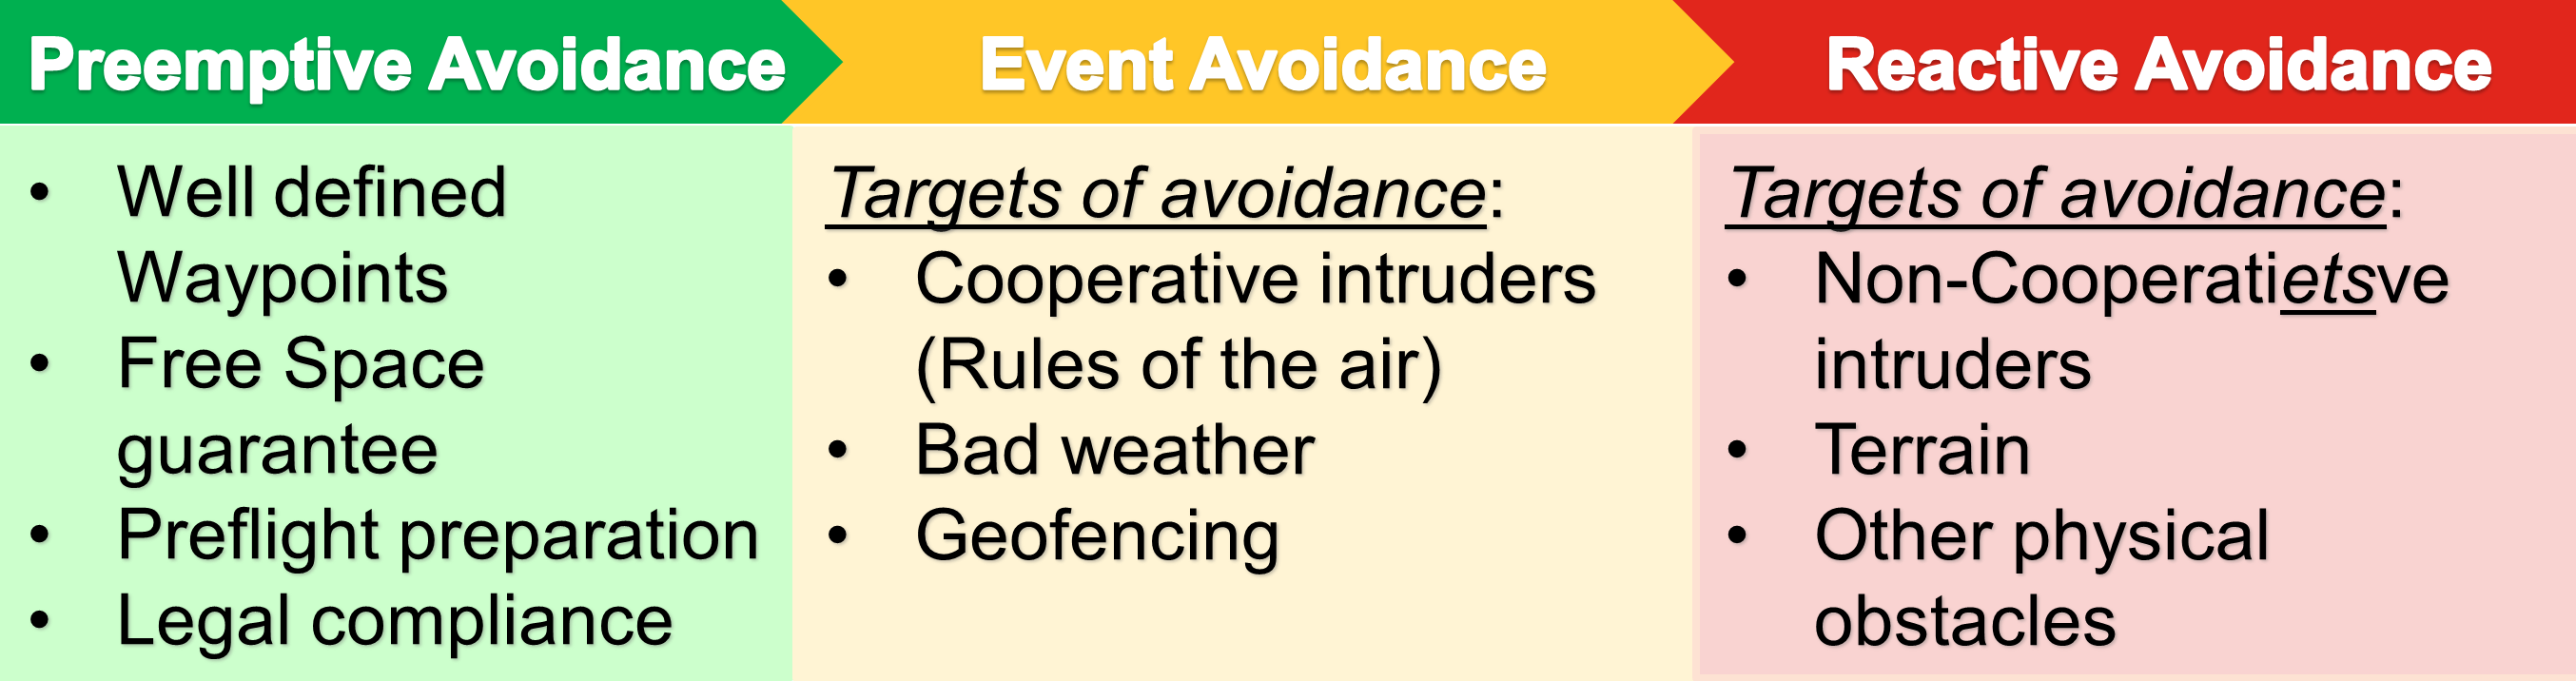
\includegraphics[width=0.7\linewidth]{\FIGDIR/RE001AvoidanceLevelsBasedOnReactionTime} 
    \caption{Avoidance levels based on reaction time.}
    \label{fig:AvoidanceLevels}
\end{figure}

\noindent This work will focus on handling \emph{Event Avoidance} and \emph{Reactive Avoidance} and the \emph{Avoidance Path} will be calculated using \emph{Reach set Based Methods}. 

The \emph{Preemptive Avoidance} is trying to remove any possible threat prior the flight. The risk mitigation is tedious and its done only when necessary. Even the best \emph{preemptive} avoidance could fail.

The \emph{Reactive Avoidance} is solving most urgent situations with very short reaction opportunity. This work focus on physical obstacles and terrain. Non cooperative intruders are partially considered. The adversary behaviour was is not considered.

The \emph{Event Avoidance} has more opportunity to react. Some threats are know prior the flight (geo-fenced areas, ...). The future UTM implementation is also considered as \emph{Event Avoidance}, due the time horizon and authority enforcement. 

\paragraph{Basic Idea:} Create deterministic finite-time \emph{Reactive Avoidance} based on \emph{Reach sets} to ensure \emph{trajectory feasibility}. Enhance method with set of the rules to enable handling more complex situations.

The \emph{Discretization} is the key to ensure calculation in finite time. Finite \emph{partition} of \emph{operational space (Known World)} and finite representation of \emph{Reach set} guarantees finite count of calculation steps. Aircraft conflict prediction mentioned in \cite{prandini2008application}.

\newpage    
\section{\secState{R}Overview}\label{s:approachOverview}

\noindent The \emph{Overview} is based on \emph{Existing} Emergency avoidance framework \cite{gomola2017obstacle} (fig. \ref{fig:avoidanceConcept}). To achieve goals defined in \emph{Problem Definition} (sec. \ref{s:BasicProblemDefinition}, \ref{s:IncrementalProblemDefinition}) following \emph{Avoidance Framework Concept} (fig. \ref{fig:AvoidanceFrameworkConceptNew}) is proposed:

\begin{figure}[H]
    \centering
    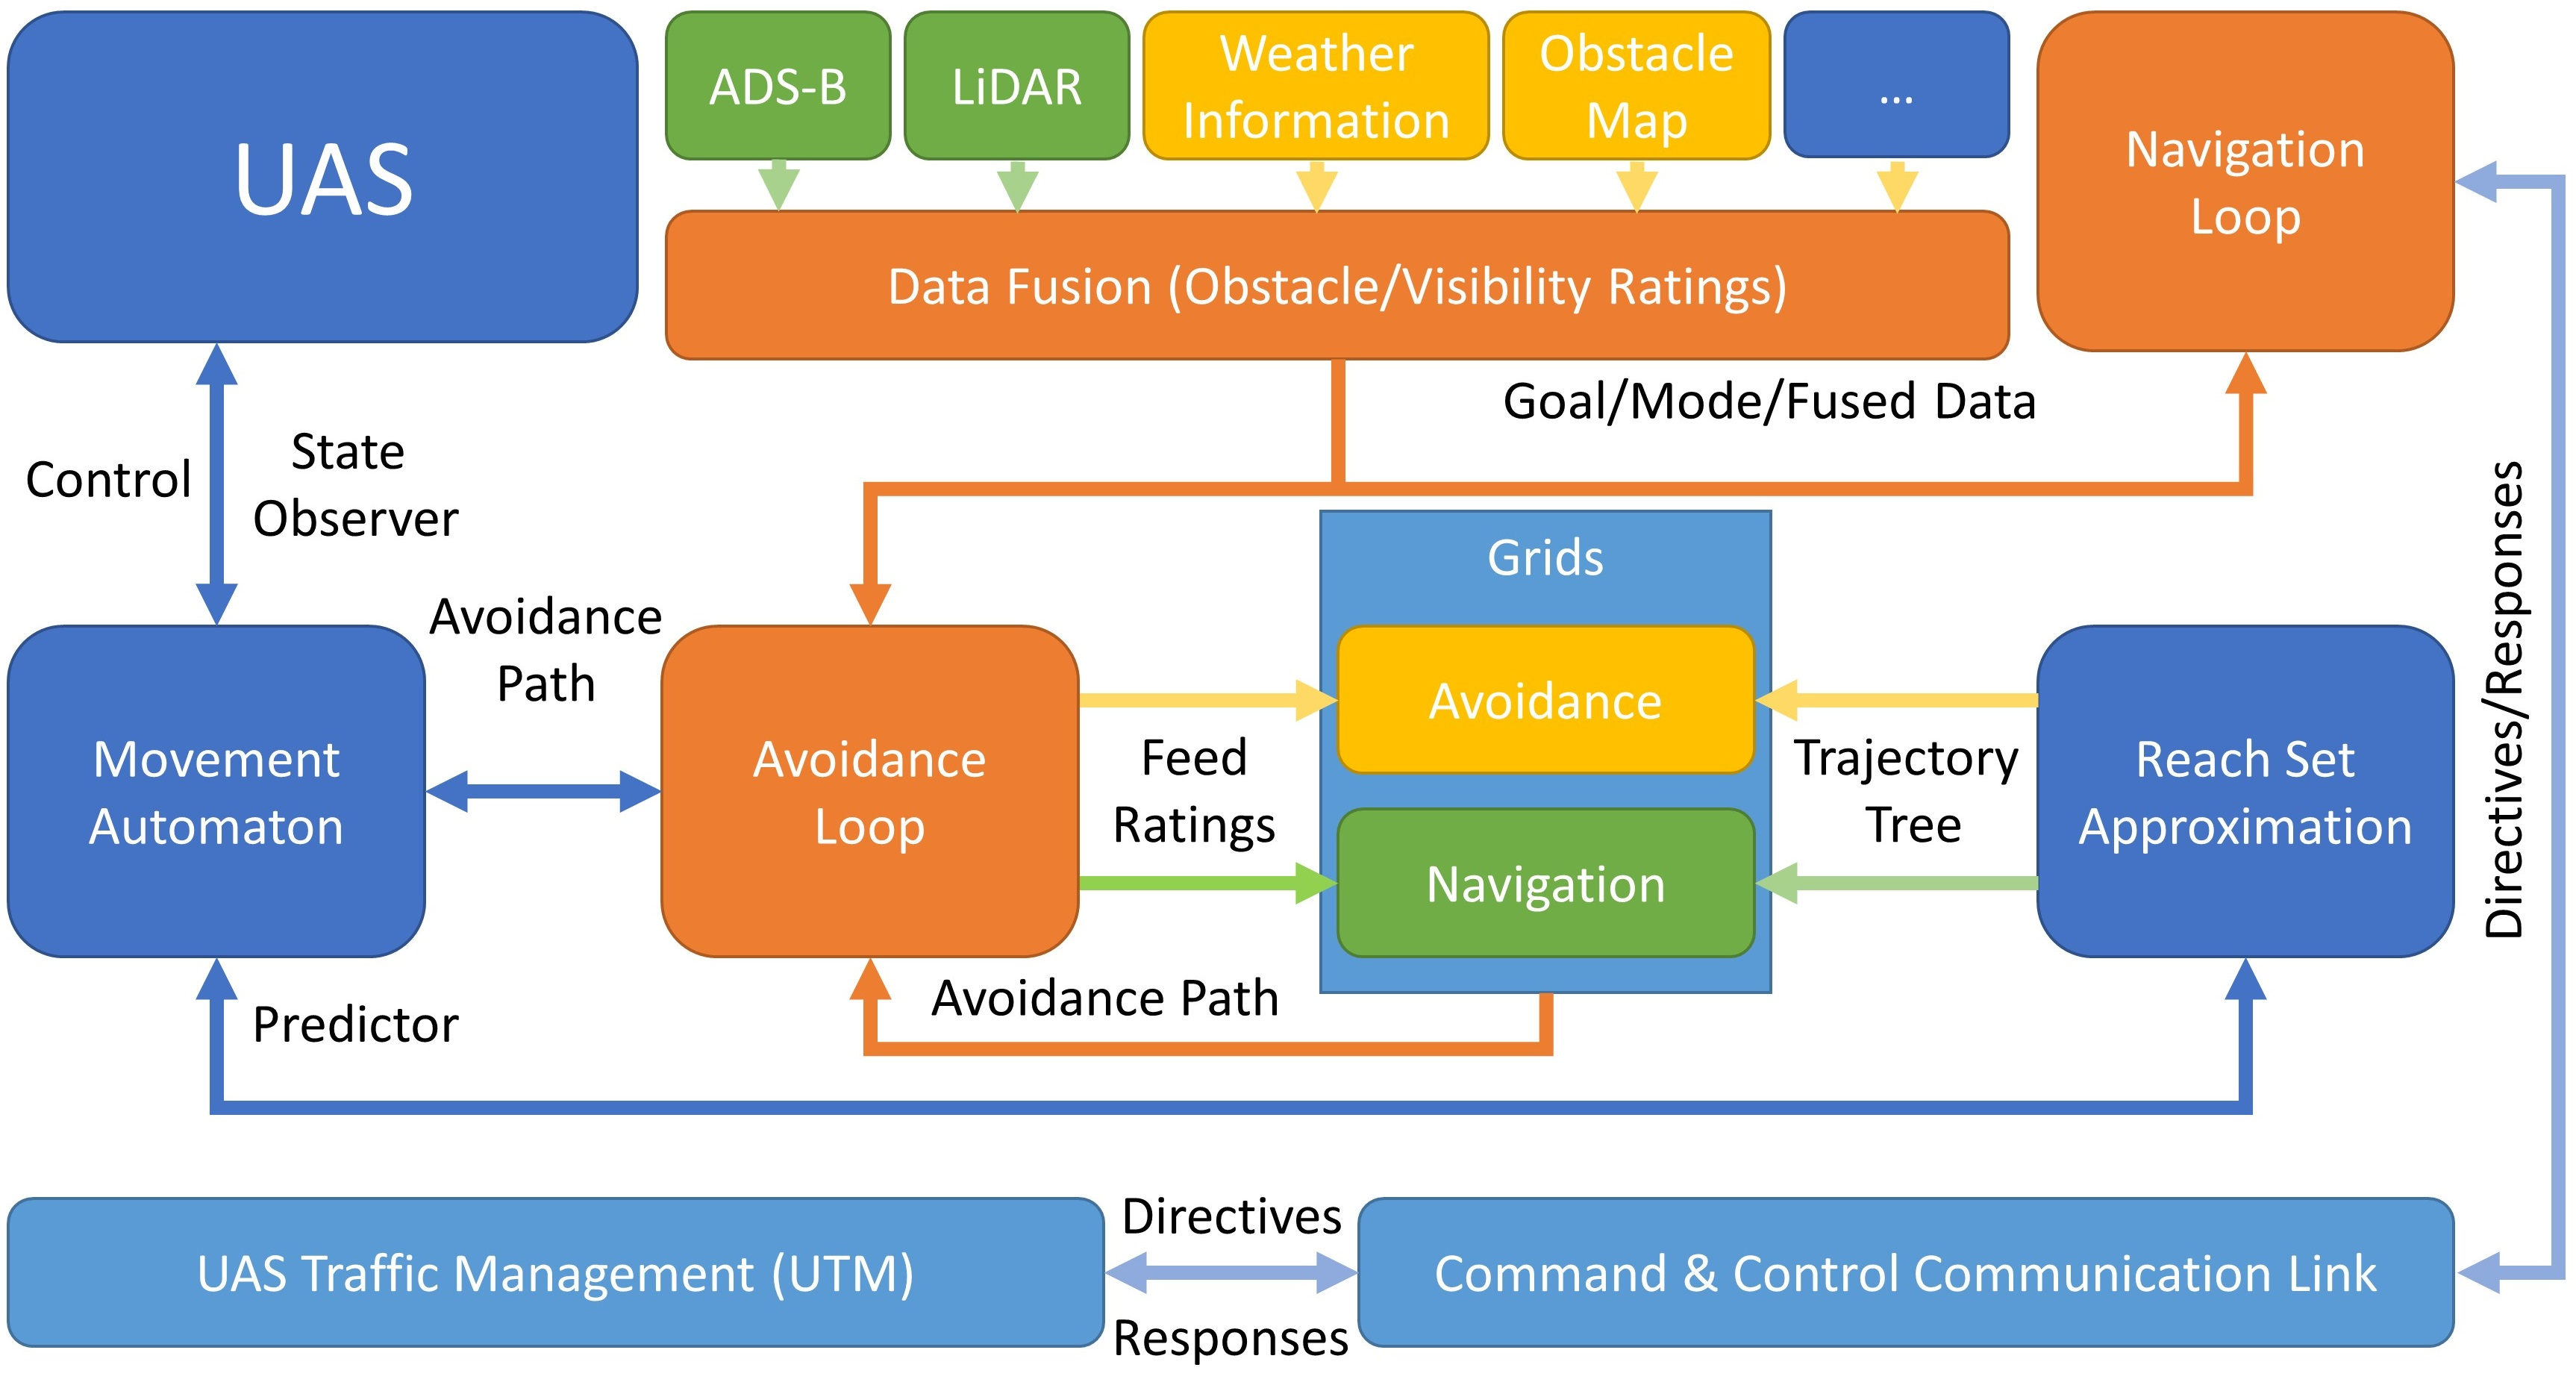
\includegraphics[width=0.95\linewidth]{\FIGDIR/TE037ConceptualSchemeNew} 
    \caption{Avoidance Framework Concept.}
    \label{fig:AvoidanceFrameworkConceptNew}
\end{figure}


\paragraph{Structure of Avoidance Framework:}

\begin{enumerate}
    \item \emph{Unmanned Aircraft System} (UAS) (Role: Controlled Plant) - the \emph{UAS} is controlled via \emph{interface} implemented as \emph{Movement Automaton}. The model used is described in (sec. \ref{s:UASNonlinearModel}).
    
    \item \emph{Movement Automaton} (Role: Control Interface/Predictor) - consumes \emph{Discrete Command Chain} to generate discrete \emph{reference trajectory}, it can be also used as a predictor of \emph{future UAS states} (sec. \ref{s:referenceTrajectoryGenerator}). The movement Automaton used in this work is given in (sec. \ref{s:movementAutomatonDefinition}). 
    
    \item \emph{Sensor Field} (Role: Surveillance Providers), following sensors were considered in this work:
        \begin{enumerate}[a.]
            \item \emph{LiDAR} (Static obstacle detection) - detection of physical obstacles (sec. \ref{s:detectedObstacles})
            
            \item \emph{ADS-B} (Intruder UAS/Plane detection) - detection of intruders whom are broadcasting their position and heading sometimes with future plans and additional parameters. The \emph{intersection models} are given in (sec. \ref{s:intruderBehaviourPrediction}, \ref{s:linearIntersectionModel}, \ref{s:bodyvolumeIntersection}, \ref{s:uncertaintyIntersection}).
        \end{enumerate}

    \newpage
    \item \emph{Information Sources} (Role: Known World Information Enhancers): 
        \begin{enumerate}[a.]
            \item \emph{Obstacle Map} (Static Restriction Source) - imposing static soft/hard constraints on \emph{Known Word}/\emph{Operational Space}. Static constraints are given in (sec. \ref{s:virtualConstraints}).
            
            \item \emph{Weather Information} (Static/Dynamic Restriction Source) - imposing static/mo\-vi\-ng soft/hard constraints on \emph{Known World}/\emph{Operational Space}. Moving constraints are given in (sec. \ref{s:MovingVirtualConstraints}).
            
            \item \emph{Other Airspace Restrictions} - like restricted airspace, geo-fencing and other future constraint sources, all of them are covered by \emph{Static/Dynamic Constraints} for now.
        \end{enumerate}
    
    \item \emph{Data Fusion} (Role: Sensor Input Interface) - is the unifying interface to asses \emph{Operational State Properties} mainly \emph{Obstacle Rating}, \emph{Visibility}, \emph{Map Obstacle Rating}, \emph{Intruder Rating} for portion of the space. The partial \emph{ratings} are proposed in related sections. The data fusion procedure with \emph{defuzzyfication} and final assessment into space sets is outlined in (sec. \ref{s:sensorFusion})  
    
    \item \emph{Reach Set Approximation} (Role: Reachability Estimator) - as \emph{data fusion} is providing the situation assessment, the \emph{Reach set} is providing maneuvering capability assessment. The introduction is given in (sec. \ref{s:reachSet}), the properties are defined in (sec. \ref{s:ReachSetPerformanceCriteria}), the approximation methods with constrained expansion are outlined in (sec. \ref{s:chaoticReachSet}, \ref{s:harmonicReachSet}, \ref{s:combinedReachSet}, \ref{s:acasReachSet}). The reach set estimation is main contribution of this work.
    
    \item \emph{Grids: Navigation/Avoidance} (Role: Operation Space Segmentation \& Situation Evaluation) - space discretization in polar coordinates grid, different reach sets are used for different grid type, defined in (sec. \ref{s:AvoidanceGrid}).
    
    \item \emph{Avoidance loop} (Role: Short Term Decision Maker) - using data from \emph{Sensor fusion} in \emph{Avoidance/Navigation Grid} trimming \emph{Reachable Space} approximated by \emph{Reach Set} generating feasible \emph{Avoidance Path}. \emph{Avoidance Path} is fed to controlling \emph{Movement Automaton}. The Goal is given by \emph{Navigation Loop}. Avoidance loop is given in (sec. \ref{s:aviudabceGridRun}).
    
    \item \emph{Navigation loop} (Role: Long Term Decision Maker) - using data from \emph{Avoidance Loop}, \emph{Mission plan} and \emph{UTM} directives defines the current long term navigation goal. Details given in (sec. \ref{s:missionControlRun}).
    
    \item \emph{Command and Control Communication Link} (C2 Link) (Role: Communication Link) - standard communication link with sufficient reliability.
    
    \item \emph{UAS Traffic Management} (UTM) (Controlled Airspace Authority) - checking possible collisions and enforces counter-measurements. Details given in (sec. \ref{sec:UASTrafficManagement}).
    
\end{enumerate}

\paragraph{Communication in Avoidance Framework:}
\begin{enumerate}
    \item \emph{UAS $\leftrightarrow$ Movement Automaton} - sharing \emph{actual system state}, commanding the UAS platform.
    
    \item \emph{Reach Set $\leftrightarrow$ Movement Automaton} - predicting set of feasible trajectories for given situation.
    
    \item \emph{Reach Set $\leftrightarrow$ Grids} - providing trajectory set depending on active mode (Navigation/Emergency Avoidance).
    
    \item \emph{Avoidance Loop $\leftrightarrow$ Data Fusion} - assessing the situation in \emph{operational space} based on sensor readings/information sources.
    
    \item \emph{Avoidance Loop $\leftrightarrow$ Navigation Loop} - determining long term goal based on situation assessment and UTM directives. 
    
    \item \emph{Avoidance Loop $\to$ Grids} - feeding assessment data and constraints into selected operational space Grid.
    
    \item \emph{Grids $\to$ Avoidance Loop} - returning feasible and \emph{cost effective} avoidance path after situation assessment and \emph{Reach set} pruning.
    
    \item \emph{Avoidance Loop $\to$ Movement Automaton} - issuing and monitoring movement commands based on actual \emph{avoidance strategy}.
    
    \item \emph{Navigation Loop $\leftrightarrow$ C2 Link $\leftrightarrow$ UTM} - communication to receive directives and send fulfillment. 
\end{enumerate}